% v2-acmsmall-sample.tex, dated March 6 2012
% This is a sample file for ACM small trim journals
%
% Compilation using 'acmsmall.cls' - version 1.3 (March 2012), Aptara Inc.
% (c) 2010 Association for Computing Machinery (ACM)
%
% Questions/Suggestions/Feedback should be addressed to => "acmtexsupport@aptaracorp.com".
% Users can also go through the FAQs available on the journal's submission webpage.
%
% Steps to compile: latex, bibtex, latex latex
%
% For tracking purposes => this is v1.3 - March 2012

\documentclass[prodmode,acmtaco]{acmsmall} % Aptara syntax


\newcommand{\pgcomment}[1]{ \par\( \clubsuit\){\bf PG: }{\rm \sf #1}\(\clubsuit\) \par}
\newcommand{\rscomment}[1]{ \par\( \clubsuit\){\bf RS: }{\rm \sf #1}\(\clubsuit\) \par}


% Package to generate and customize Algorithm as per ACM style
%\usepackage[ruled]{algorithm2e}
%\renewcommand{\algorithmcfname}{ALGORITHM}
%\SetAlFnt{\small}
%\SetAlCapFnt{\small}
%\SetAlCapNameFnt{\small}
%\SetAlCapHSkip{0pt}
%\IncMargin{-\parindent}

% Metadata Information
\acmVolume{9}
\acmNumber{4}
\acmArticle{39}
\acmYear{2016}
\acmMonth{3}

% Copyright
%\setcopyright{acmcopyright}
%\setcopyright{acmlicensed}
%\setcopyright{rightsretained}
%\setcopyright{usgov}
%\setcopyright{usgovmixed}
%\setcopyright{cagov}
%\setcopyright{cagovmixed}

% DOI
\doi{0000001.0000001}

%ISSN
\issn{1234-56789}

% Document starts
\begin{document}

% Page heads
\markboth{P. Garcia et al.}{Statistical Optimisations of Asynchronous Dynamic Dataflow}

% Title portion
\title{Statistical Optimisations of Asynchronous Dynamic Dataflow}
\author{Paulo Garcia
\affil{Heriot-Watt University}
Robert Stewart
\affil{Heriot-Watt University}
}
% NOTE! Affiliations placed here should be for the institution where the
%       BULK of the research was done. If the author has gone to a new
%       institution, before publication, the (above) affiliation should NOT be changed.
%       The authors 'current' address may be given in the "Author's addresses:" block (below).
%       So for example, Mr. Abdelzaher, the bulk of the research was done at UIUC, and he is
%       currently affiliated with NASA.

\begin{abstract}

Pr

\end{abstract}


%
% The code below should be generated by the tool at
% http://dl.acm.org/ccs.cfm
% Please copy and paste the code instead of the example below. 
%
 \begin{CCSXML}
<ccs2012>
<concept>
<concept_id>10010583.10010600.10010628</concept_id>
<concept_desc>Hardware~Reconfigurable logic and FPGAs</concept_desc>
<concept_significance>500</concept_significance>
</concept>
<concept>
<concept_id>10010583.10010682.10010684</concept_id>
<concept_desc>Hardware~High-level and register-transfer level synthesis</concept_desc>
<concept_significance>500</concept_significance>
</concept>
<concept>
<concept_id>10010583.10010682.10010689</concept_id>
<concept_desc>Hardware~Hardware description languages and compilation</concept_desc>
<concept_significance>500</concept_significance>
</concept>
<concept>
<concept_id>10010583.10010682.10010690</concept_id>
<concept_desc>Hardware~Logic synthesis</concept_desc>
<concept_significance>500</concept_significance>
</concept>
<concept>
<concept_id>10011007.10011006.10011008</concept_id>
<concept_desc>Software and its engineering~General programming languages</concept_desc>
<concept_significance>500</concept_significance>
</concept>
<concept>
<concept_id>10011007.10011006.10011060.10011062</concept_id>
<concept_desc>Software and its engineering~Architecture description languages</concept_desc>
<concept_significance>500</concept_significance>
</concept>
</ccs2012>
\end{CCSXML}

\ccsdesc[500]{Hardware~Reconfigurable logic and FPGAs}
\ccsdesc[500]{Hardware~High-level and register-transfer level synthesis}
\ccsdesc[500]{Hardware~Hardware description languages and compilation}
\ccsdesc[500]{Hardware~Logic synthesis}
\ccsdesc[500]{Software and its engineering~General programming languages}
\ccsdesc[500]{Software and its engineering~Architecture description languages}

%
% End generated code
%

% We no longer use \terms command
%\terms{Design, Algorithms, Performance}

%\keywords{Wirele}

\acmformat{Paulo~Garcia, Robert~Stewart. Statistical Optimisations of Asynchronous Dynamic Dataflow}
% At a minimum you need to supply the author names, year and a title.
% IMPORTANT:
% Full first names whenever they are known, surname last, followed by a period.
% In the case of two authors, 'and' is placed between them.
% In the case of three or more authors, the serial comma is used, that is, all author names
% except the last one but including the penultimate author's name are followed by a comma,
% and then 'and' is placed before the final author's name.
% If only first and middle initials are known, then each initial
% is followed by a period and they are separated by a space.
% The remaining information (journal title, volume, article number, date, etc.) is 'auto-generated'.

\begin{bottomstuff}
This work is supported by 
\end{bottomstuff}

\maketitle




\section{Introduction}

The dataflow model(s) of computation is a paradigm that can be used to implement, represent and reason about myriad processes. Dataflow models processes as concurrent computational blocks (actors) communicating through data (tokens) sent across point-to-point channels. This paradigm is applicable to hardware pipelines, parallel software, distributed systems, etc.; and has been used to implement a broad range of solutions, using one of the many dataflow sub-models, depending on the nature of the application. 
\par The different models of dataflow differ in two key areas: synchronicity and token throughput. \textit{Synchronicity} refers to the timing semantics of different actors: are their actions scheduled according to a global time frame, which can be predicted statically? Or are execution semantics unpredictably variable throughout runtime? \textit{Token throughput} refers to token consumption and production rates: do actors consume/produce a fixed number of tokens per action (or cyclic sequences of tokens), which can be used to reason about global throughput? Or is the throughput unpredictable as well? 
\par There is an inversely proportional relation between predictability and applicability. The simplest models, which exhibit highly predictable execution semantics, can be used to design and represent equally simple systems: e.g., synchronous state-less hardware. The most complex model -dynamic asynchronous- can be used to design and represent virtually any system at any scale (e.g., distributed computing), at the cost of predictability: i.e., it is more complex to reason about its execution semantics, namely timing.
\par Timing analysis, however, is of paramount importance to \textit{optimisation functions}: manual or automated methods that consume a dataflow network and produce and optimised version. Re-designing or refactoring a dataflow system to optimise a particular metric (e.g., performance, power consumption) requires trustworthy assumptions about the behaviour of that system. State of the art timing analysis methodologies, however, are based on formal semantics that rely on static token throughput and synchronisation. 
\par In this paper, we investigate the timing analysis of dynamic asynchronous dataflow and its application to optimisation functions. We abandon the notion of precise timing knowledge, and instead build statistical timing models that can guide optimisation functions. Specifically, this paper offers the following contributions:

\begin{itemize}
\item We identify and discuss the limitations of state of the art timing analysis techniques for asynchronous dynamic dataflow, and how these limitations prevent optimisations across a broad range of dataflow implementations.
\item We present a methodology for statistical timing analysis based on Probablity Density Functions (PDFs), which can be applied to asynchronous dynamic dataflow.
\item We present a methodology that applies PDF analysis to dataflow optimisations, namely scheduling strategies for software implementations and clock gating strategies for hardware implementations.
\end{itemize}

\par The remainder of this paper is organized as follow: in Section \ref{sec:back}, we revise the different types of dataflow models and the state of the art in dataflow timing analysis, and highlight the current limitations of applying such techniques to asynchronous dynamic dataflow. In Section \ref{sec:pdf}, we present our methodology for statistical timing analysis of asynchronous dynamic dataflow. In Section \ref{sec:sched}, we describe how our timing analysis can be applied to scheduling optimisations of dataflow software implementations, and in Section \ref{sec:gate} we describe how it can be applied to clock gating optimisations of dataflow hardware implementations. In Section \ref{sec:exp}, we evaluate our approaches on a suite of dataflow applications, implemented on CPU and FPGA. Finally, we present our conclusions and identify future work in Section \ref{sec:conc}. 




\section{Background and Related Work}\label{sec:back}

In order to have this paper self-contained, we review three dataflow models: static synchronous, cyclo-static synchronous, and dynamic asynchronous (the interested reader may refer to \cite{7094787} and \cite{Bouakaz:2017:SPD:3029795.2999539} for a more detailed discussion of other models such as cyclo-static asynchronous). Although other model variants exist, we focus our expos\'{e} on these three types, which suffice to illustrate the key aspects of interest in this paper. 




\begin{itemize}
\item different types of dataflow, focusing on dynamic asynchronous
\item related work in timing estimation, token critical path analysis
\item examples of why it doesn't work for dynamic asynchronous
\end{itemize}


\section{PDF critical path analysis}\label{sec:pdf}


As previously mentioned, the timing analysis of synchronous dataflow is predicated on predictable token consumption/production rates at discrete, globally synchronised points in time. This discrete scheduling may be a global clock transition in hardware implementations or a scheduling time slice in software implementations. On asynchronous dataflow, this discrete abstraction must be abandoned: absolute continuous time must instead be adopted. This is true even in Globally Asynchronous Locally Synchronous (GALS) hardware implementations: even though each actor operates under its own (discrete) clock, clock frequencies may be completely unrelated in frequency and phase. The goal of PDF analysis is to obtain a token throughput timing profile in absolute time, under unpredictable token consumption/production rates. This is done through network profiling, collecting runtime statistics about each actor's behaviour.

\subsection{Single Input Single Output Actors}

\begin{figure}[tb]
  \centering
  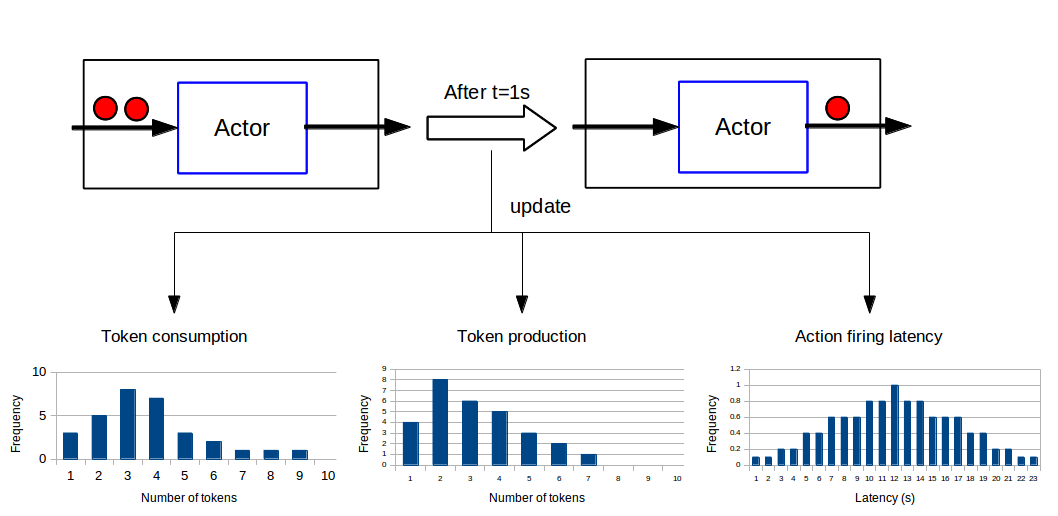
\includegraphics[width=1\columnwidth]{img/example1.png}
  \caption{Profile update after action firing: token consumption is updated by incrementing bin 2, token production is updated by incrementing bin 1, and latency is is updated by incrementing bin 1. Histogram shapes are purely illustrative.}
  \label{fig:example1}
\end{figure}




For the simplest possible dynamic asynchronous actor, with one input and one output port, we monitor how many tokens are consumed and produced per action firing, and how long it takes between successive action firings, assuming sufficient input tokens are always available. It should be noted that we assume these two metrics to be independent: the dynamic nature of actors doen't allow for any assumptions of correlation between token consumption and latency. Fig. \ref{fig:example1} depicts an example of such profiling, for different token throughput and action latencies, and examples of histograms for each metric.



\par In order to model actors' behaviour in absolute continuous time, 

\begin{itemize}
\item each actor latency (avg of actions) as a PDF
\item effect of pipeline analysis of PDF
\item effect of feedback loops analysis of PDFs
\end{itemize}



\section{Scheduling strategies}\label{sec:sched}

\begin{itemize}
\item Assuming round robin scheduling
\item Counters to determine where to move to
\end{itemize}


\section{Gating strategies}\label{sec:gate}

\begin{itemize}
\item Timers to determine when to gate
\end{itemize}


\section{Experiments}\label{sec:exp}
\section{Conclusions}\label{sec:conc}













% Acknowledgments
\begin{acks}
We acknowledge the support of the Engineering and Physical Research
Council, grant references EP/K009931/1 (Programmable embedded
platforms for remote and compute intensive image processing
applications) and EP/J015180/1 (Sensor Signal Processing).
\end{acks}

% Bibliography
\bibliographystyle{ACM-Reference-Format-Journals}
\bibliography{references}
                             % Sample .bib file with references that match those in
                             % the 'Specifications Document (V1.5)' as well containing
                             % 'legacy' bibs and bibs with 'alternate codings'.
                             % Gerry Murray - March 2012

% History dates
\received{February 2016}{March 2016}{June 2016}


\end{document}
% End of v2-acmsmall-sample.tex (March 2012) - Gerry Murray, ACM


